
 
 %__________________________________________________________
 \chapter{Software development}
 
 
 \section{Software development life cycle} 
 
 
 
 \usetikzlibrary{shapes.geometric, arrows}
 
 \usetikzlibrary{positioning} 
 
 \tikzstyle{block} = [draw, rectangle, rounded corners, draw=black, very thick,
 fill={rgb:orange,1;yellow,2;pink,5},
 text width=4cm, text centered, minimum height=1.2cm, node distance=3cm]
 \tikzstyle{container} = [draw, rectangle, inner sep=0.3cm]
 
 \tikzstyle{text} = [draw, color=blue]
 \tikzstyle{arrow} = [thick,->, >=latex]
 \tikzstyle{line} = [thick,-]
 
 
 \begin{figure}[]
 	\centering
 	
 	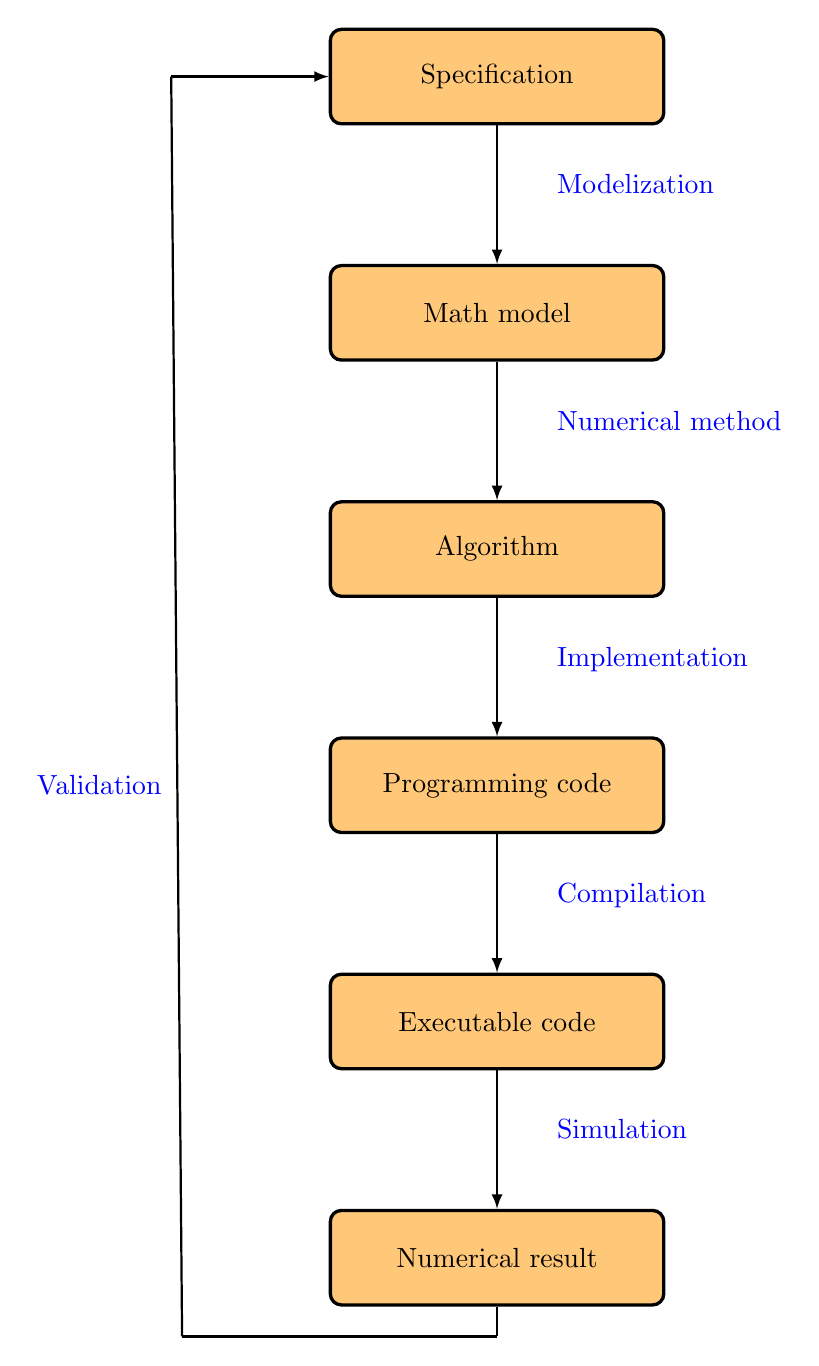
\begin{tikzpicture}
 	
 	\node [block, name=s] {Specification};
 	\node [block, below of=s] (m) {Math model} ;
 	\node [block, below of=m] (a) {Algorithm};
 	\node [block, below of=a] (p) {Programming code};
 	\node [block, below of=p] (e) {Executable code};
 	\node [block, below of=e] (r) {Numerical result};
 	
 	\node [coordinate, below of=r] (d1) {};
 	\node [coordinate, left=3cm and 4cm of d1] (d2) {};
 	\node [coordinate, left=1cm and 2cm of s] (d3) {};
 	
 	
 	\draw [arrow] (s) -- (m);
 	\draw [arrow] (m) -- (a);
 	\draw [arrow] (a) -- (p);
 	\draw [arrow] (p) -- (e);
 	\draw [arrow] (e) -- (r);
 	
 	\draw [line] (r) -- (d1);
 	\draw [line] (d1) -- (d2);
 	\draw [line] (d2) -- (d3);
 	\draw [arrow] (d3) -- (s);
 	
 	\node [color=blue, left=1cm and 2cm of p] (v) {Validation};
 	%  \node [coordinate=0cm and 1cm of s] (m) {Model};
 	
 	\node [color=blue, below right=0.5cm and -1.5cm of s ]  {Modelization};
 	\node [color=blue, below right=0.5cm and -1.5cm of m ]  {Numerical method};
 	\node [color=blue, below right=0.5cm and -1.5cm of a ]  {Implementation};
 	\node [color=blue, below right=0.5cm and -1.5cm of p ]  {Compilation};
 	\node [color=blue, below right=0.5cm and -1.5cm of e ]  {Simulation};
 	
 	
 	\end{tikzpicture}
 	
 	\caption{Software Development Life Cycle }
 \end{figure}



\newpage
\section{Methodology}

\subsection{Names of function, classes and variables} 
\begin{itemize} 
	\item Snake case
	
	\item Camel case. 
	
	
	\item Upper case : classes and ... 
	
	\item Indentation.   
	
	
	\item max length. 
	
	
\end{itemize}


\subsection{Code developing methodology} 
\begin{itemize} 
	\item Top--down. functional paradigm. multi-layer and multi-group decomposition. 
	
	\item Xtreme programming. Driver: write the code. Reviewer: ask questions. Unit testing. 
	      Every function a validation program. 
	
	\item Continuation techniques. 
	
	\item Test Driven Development.  
	   \begin{enumerate}
	   	 \item Design a write a test. 
	   	 \item Write the code. 
	   	 \item Run the test and verify. 
	   	 \item Refactoring the code. clean up. 
	   	 \item Repeat and start new test.  
	   	\end{enumerate} 
   	Mantra: RED (fail), GREEN(pass), REFACTOR 
	
	\item Axiomatic design. max independence. minimum information content. customer needs -- functional requirements. 
	

\end{itemize} 

Duplication is prohibited. 

Object class represents its purpose. 



 
 
 
 
 

